\section{Theoretical Background}


\subsection{Visual Information Processing}

\begin{frame}
\frametitle{Visual Information Processing}
	\begin{columns}
		\begin{column}{0.5\textwidth}
			\begin{itemize}
				\uncover<1->{\item Visual information route from the eyes to the visual cortex}
				\uncover<2->{\item Distinction based on motion}
				\uncover<3->{\item Assigned to category-specific information processing centers}
			\end{itemize}
		\end{column}

		\begin{column}{0.49\textwidth}
			\only<1>{
				\begin{figure}
					\centering
					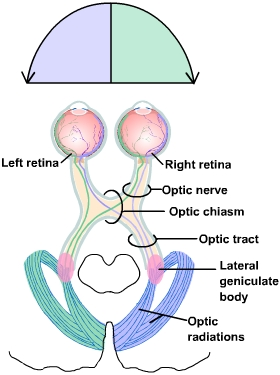
\includegraphics[width=0.98\textwidth, height=6cm]{assets/Optic_Pathway.jpg}
					\caption*{Visual Information Flow to V1}
				\end{figure}
				}
			\only<2>{
				\begin{figure}
					\centering
					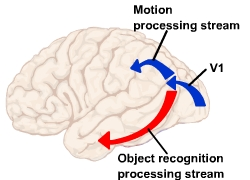
\includegraphics[width=0.98\textwidth]{assets/Info_distinction_from_vis_cortex.jpg}
					\caption*{Ventral and Dorsal Information Streams}
				\end{figure}
				}
			\only<3>{
				\begin{figure}
					\centering
					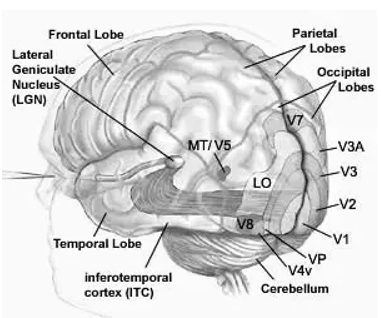
\includegraphics[width=0.98\textwidth]{assets/visual_areas.png}
					\caption*{Brain Region Specialization Regarding Visual Information Processing}
				\end{figure}
				}
		\end{column}
	\end{columns}
\end{frame}

\begin{frame}
\frametitle{Category-Specific Information Processing Centers}
	\begin{itemize}
		\uncover<1>{\item Fusiform Face Area - Occipital Face Area\\Parahippocampal Place Area - Latteral Occipital Cortex\\Extrastriate Body Area - Fusiform Body Area}
	\end{itemize}
	\begin{figure}
		\centering
		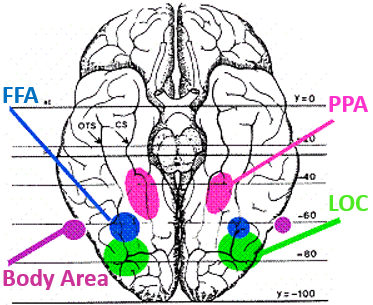
\includegraphics[width=0.9\textwidth, height=6cm]{assets/brain_areas.png}
	\end{figure}
\end{frame}


\subsection{Mechanisms of fMRI}

\begin{frame}
\frametitle{NMR Signal}
	\begin{itemize}
		\uncover<1->{\item Scanner generates a powerful magnetic field $\vec{B_0}$}
		\uncover<2->{\item Magnetic moments of nonzero spin nuclei\\(protons - water) weakly align with $\vec{B_0}$,\\creating a net macroscopic magnetization $\vec{M_0}$}
		\uncover<3->{\item Coil transmits RF transverse magnetic field pulse\\at resonant frequency tipping $\vec{M_0}$ from alignment}
		\uncover<4->{\item $\vec{M_0}$ precesses around $\vec{B_0}$ to return to equilibrium}
		\uncover<5->{\item Rotating $M_{\text{xy}}$ component generates oscillating magnetic field\\inducing current, producing signal}
	\end{itemize}
\end{frame}


\begin{frame}
\frametitle{T1 Relaxation}
	\begin{itemize}
		\uncover<1->{\item The process by which the $z$ component of the net magnetization $M$ returns to its initial maximum value $M_0$ parallel to $B_0$}
		\vspace{1.2cm}
		\uncover<2->{\item Measured T1, modified by blood inflow relocating spins\\in-and-out of the imaging plane, is termed T1*}
	\end{itemize}
	\begin{figure}
		\centering
		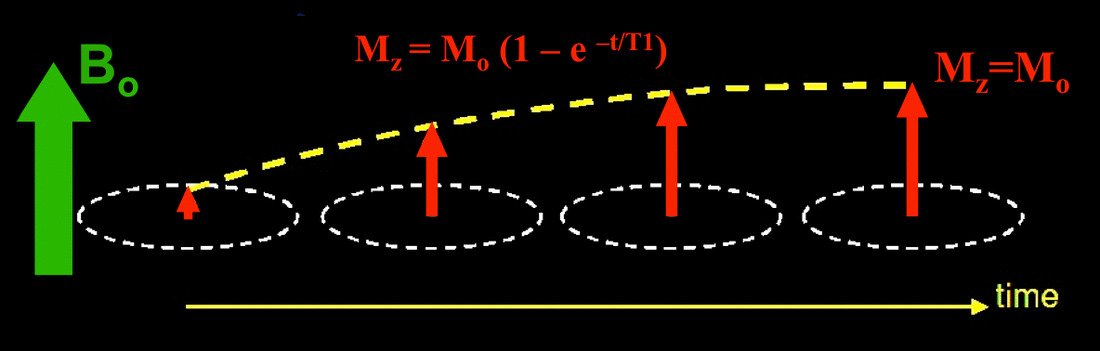
\includegraphics[width=0.98\textwidth]{assets/T1_illustration.jpg}
		\caption*{Illustration of T1 Relaxation}
	\end{figure}
\end{frame}

% Mention T1* briefly

\begin{frame}
\frametitle{T2 Relaxation}
	\begin{itemize}
		\uncover<1>{\item T2 is the time constant for dephasing of trasverse magnerization $M_{\text{xy}}$}
		\vspace{1.5cm}
		\uncover<2->{\item Following an RF pulse spin distribution is conserved,\\from the $z$ axis to phase coherence in the $\text{xy}$ plane,\\leading to precession of spins at the Larmor frequency}
	\end{itemize}
	\begin{figure}
		\centering
		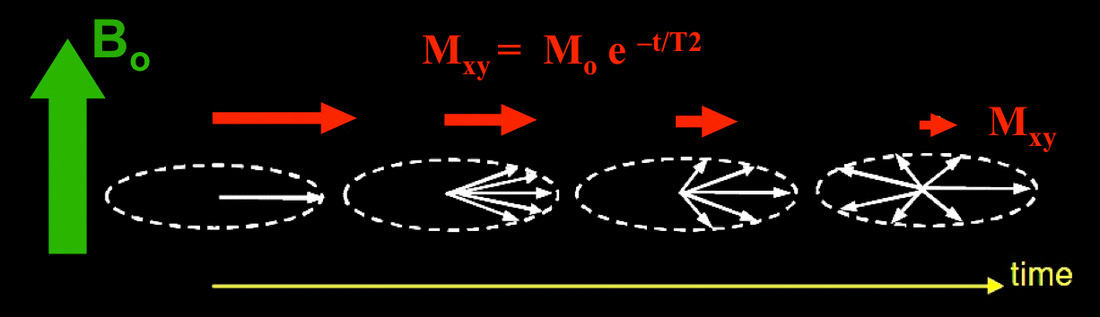
\includegraphics[width=0.98\textwidth]{assets/T2_illustration.jpg}
		\caption*{Illustration of T2 Relaxation}
	\end{figure}
\end{frame}


\begin{frame}
\frametitle{T2* Relaxation}
	\begin{figure}
		\centering
		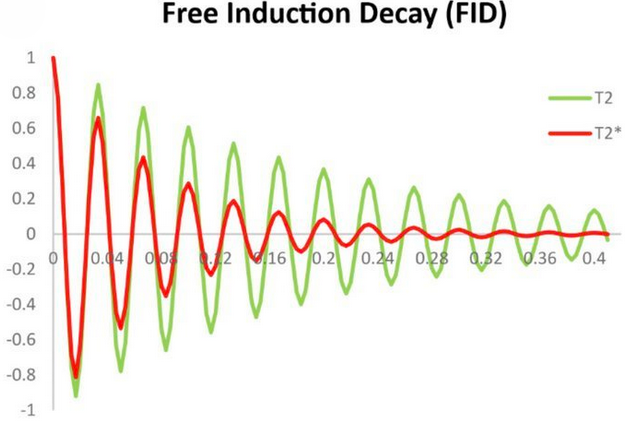
\includegraphics[width=0.98\textwidth, height=5cm]{assets/FID.png}
	\end{figure}
	\begin{itemize}
		\uncover<1>{\item "Effective" T2* is much shorter than "natural" T2\\due to inhomogeneities in the main magnetic field}
	\end{itemize}
\end{frame}


\begin{frame}
\frametitle{BOLD Signal}
	\begin{columns}
		\begin{column}{0.4\textwidth}
			\begin{itemize}
				\uncover<1->{\item Blood Oxygen-Level Dependent Signal}
				\uncover<2->{\item Detects changes in HbR driven by localized changed in blood flow and blood oxygenation}
				\uncover<3->{\item HbR is paramagnetic, making it a naturally occurring contrast agent}
				\uncover<4->{\item Neural activity reduces the OEF which increases MR signal locally}
			\end{itemize}
		\end{column}
		
		\begin{column}{0.59\textwidth}
			\only<1->{
				\begin{figure}
					\centering
					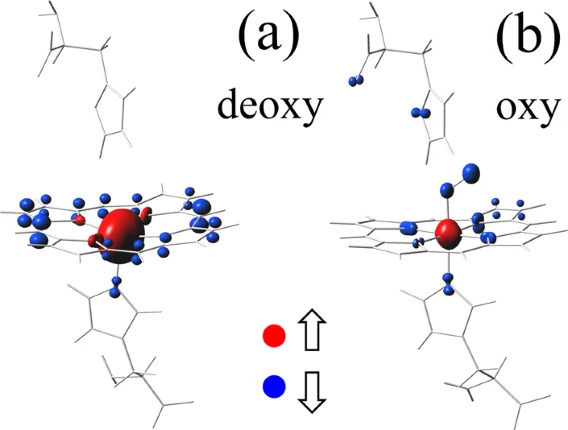
\includegraphics[width=0.98\textwidth]{assets/DeoxyHb_magnetic.jpg}
					\caption*{Illustration of Oxyhemoglobin and Deoxyhemoglobin Magnetic Moment Density}
				\end{figure}
				}
		\end{column}
\end{columns}
\end{frame}


\begin{frame}
\frametitle{BOLD Response}
	\begin{figure}
		\centering
		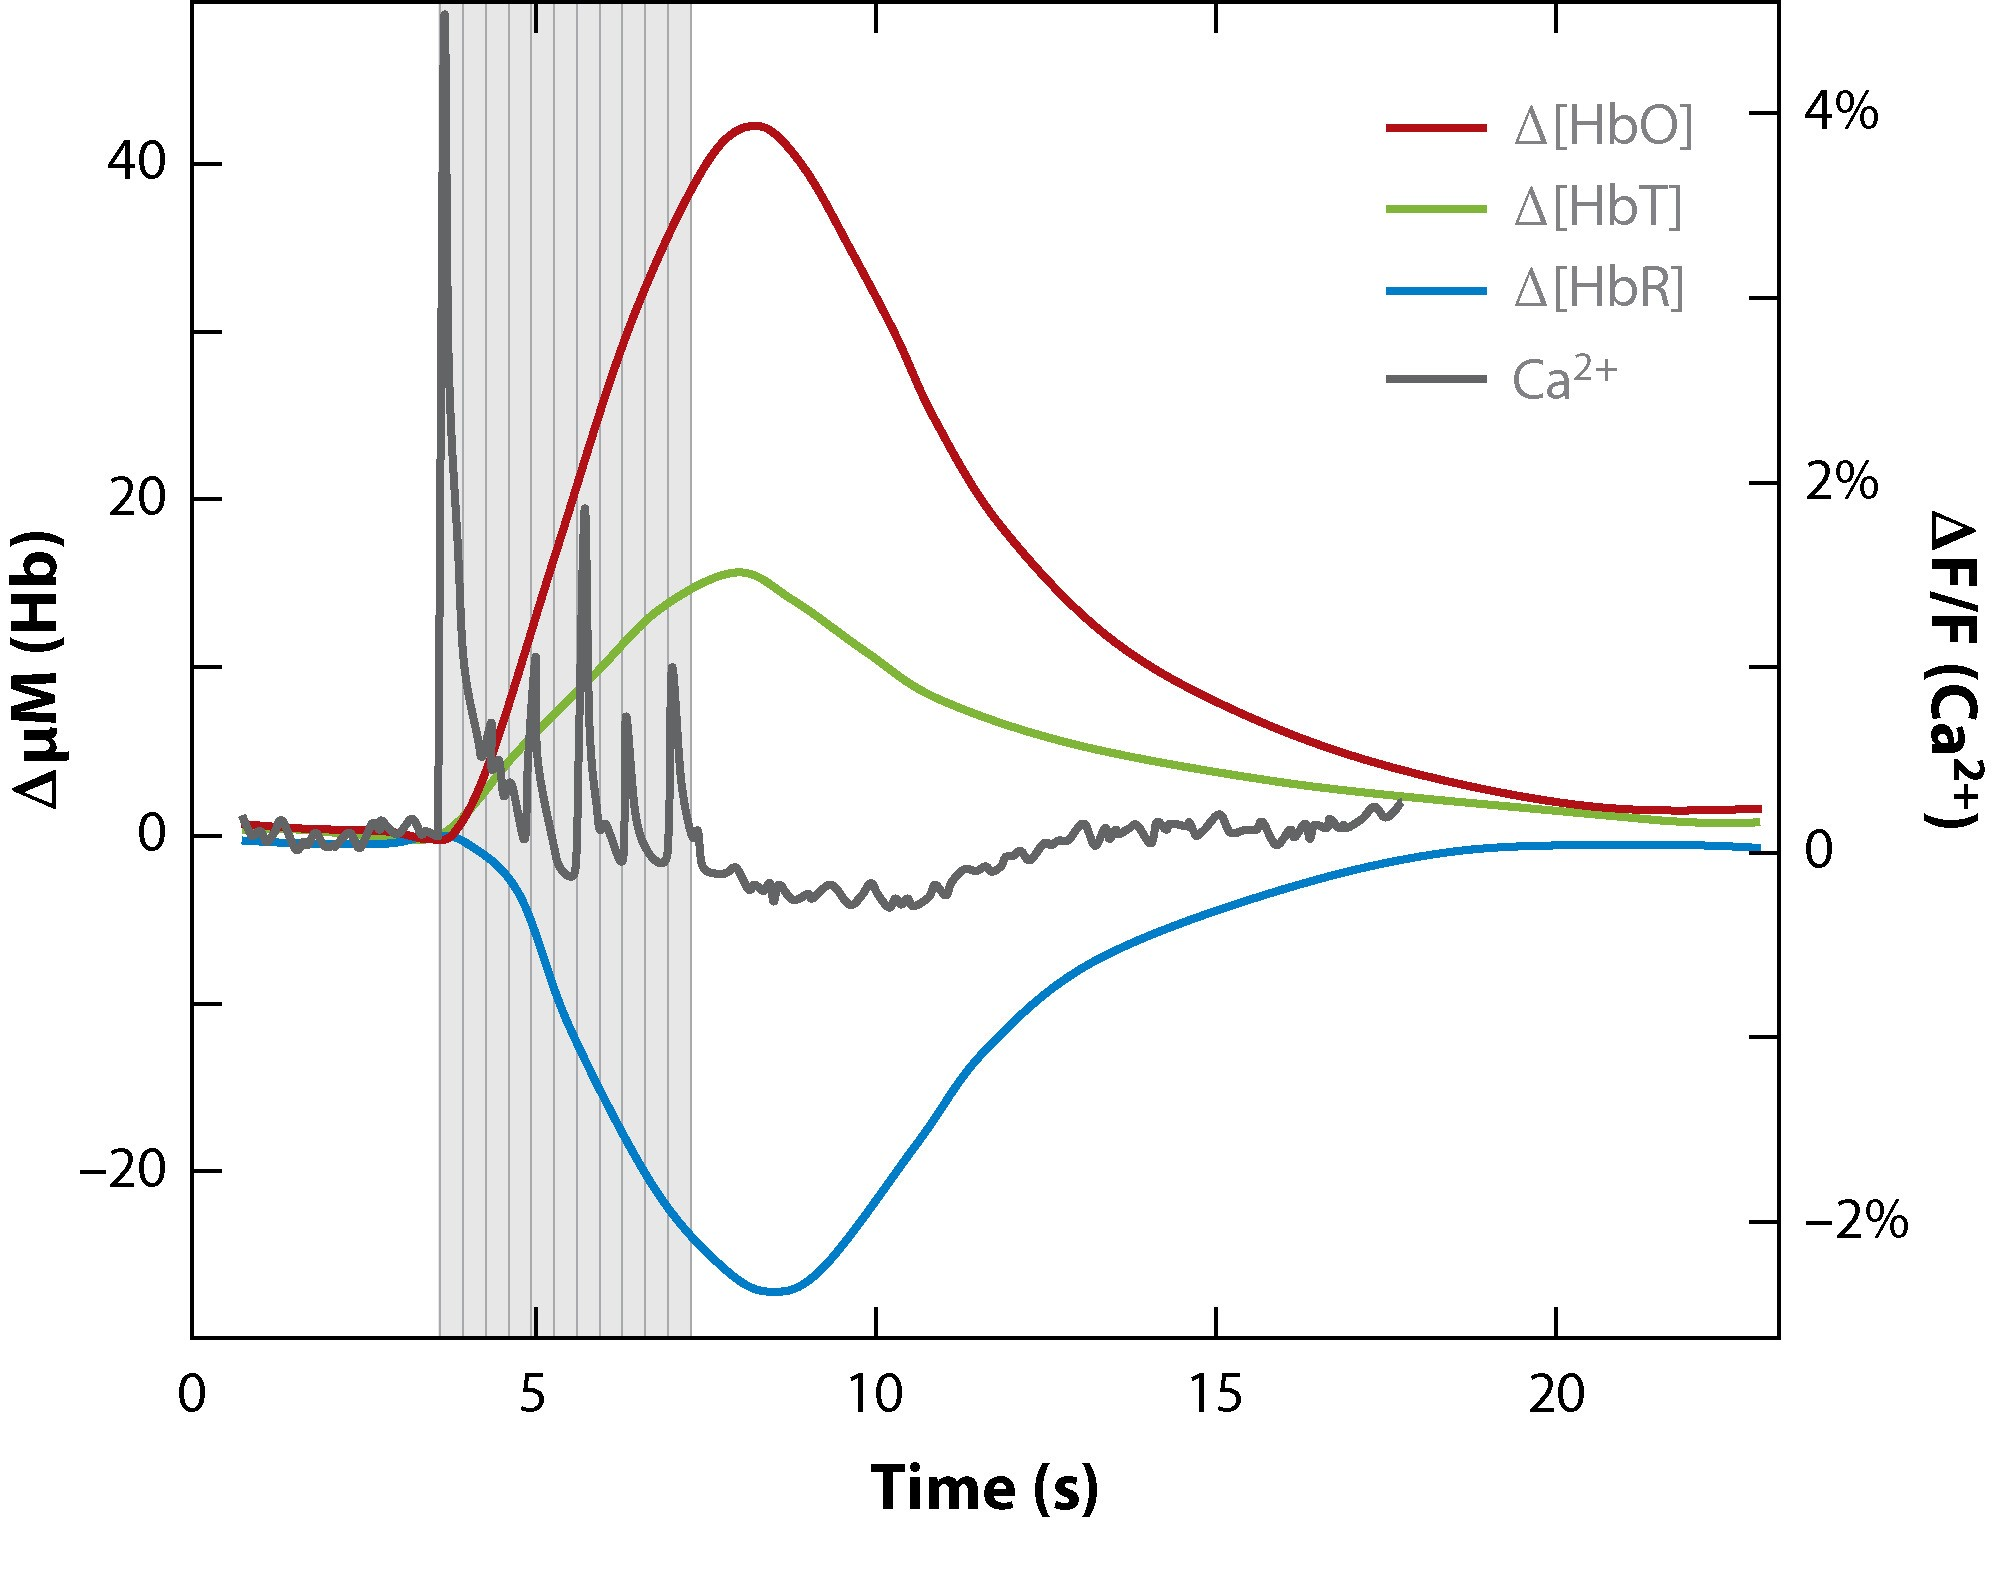
\includegraphics[width=0.98\textwidth, height=7cm]{assets/Hb_flactuations_BOLD.jpg}
		\caption*{Stimulus-Evoked Response in Somatosensory Cortex of Rats}
	\end{figure}
\end{frame}